\documentclass[12pt]{article}
\usepackage{graphicx}
\usepackage{geometry}
\usepackage{fancyhdr}
\usepackage{titletoc}
\usepackage{titlesec}
\usepackage{listings}
\usepackage{float}

% Page setup
\geometry{
    top=1in,
    bottom=1in,
    left=1in, % Adjust the left margin
    right=1in, % Adjust the right margin
}

% breaklines=true,

\pagestyle{fancy}
\fancyhf{} % Clear all header and footer fields
\fancyhead[R]{Reflection and Assessment Plan} % Add this line to set the header on the right side
\renewcommand{\headrulewidth}{0pt} % Remove the horizontal line in the header

% Define section numbering format
\titleformat{\section}{\normalfont\large\bfseries}{\thesection}{1em}{}
\titleformat{\subsection}{\normalfont\normalsize\bfseries}{\thesubsection}{1em}{}

% Title Page
\begin{document}
\begin{titlepage}
    \centering
    {\LARGE\textbf{EE/CE 468: Mobile Robotics}\par}
    \vspace{0.5cm}
    {\Large Reflection and Assessment Plan\par}
    \vspace*{\fill} % Vertically center the logo and text
    {\large Muhammad Azeem Haider $\mid$ mh06858@st.habib.edu.pk\par}
    \vspace{2cm}
    
\includegraphics[height=7cm]{../HU_logo.png}\\\bigskip
    {\large \today}\\\bigskip\bigskip
    \vspace{2cm}
    {\large Dhanani School of Science and Engineering\par}
    {\large Habib University\par}
    {\large Fall 2023\par}
    \vspace*{\fill} % Vertically center the copyright text
    {\large Copyright @ 2023 Habib University\par}
\end{titlepage}

% Index page
\thispagestyle{empty} % No page number on the index page
% \tableofcontents
\clearpage

\section{Understanding Fundamental Concepts of Mobile Robotics}

At the start of the course, in my first quiz I got a 31.5/100. This was a big
setback especially considering I actually studied for the course but despite my
efforts, the results showed gaps in my knowledge and understanding. Over the
course of the semester, I have improved my quiz grades, and that is something I
believe is a proof of better understanding of fundamental concepts of mobile
robotics. While I by no means mean that the improvement in my quiz grades is a
sure-fire proof of my understanding of the fundamental concepts of mobile
robotics, I do believe that it is a good indicator, and I can build on this
improvement. The practical implementation of the robotics project was carried
out in different phases. The first step was to come up with a strategy in
theoretical realms and then look for literature based on that strategy. While
we did not find much literature on random walk, we did find a couple of good
research papers comparing different random walk algorithms for coverage
problem. I implemented random walk strategies in Matlab and the strategy grew
into a more sophisticated spiral random walk algorithm which can be seen in the
results. \newline \\ While I was unable to take journal notes, I want to talk
about how the understanding of fundamental concepts help me grow interest in
the course. From almost withdrawing from the course at one point, going through
the books to better understand simple concepts such as frames of reference and
kinematic model helped me alot, these simple concepts built one upon another
and helped bring the course to a happy end for me in terms of learning albeit
it does not very successfully translate in terms of grades. I believe that
project outcome was successful in terms of learning. While we were unable to
implement a super complex coverage algorithm, we implemented a simple algorithm
that does the same thing and created a strategy on our own. I am not entirely
sure what grade I would give myself because of the varying factors in this
goal, but I am happy with how I have grown as a mobile robotics student.

\section{Improving Matlab and Robotics Programming Skills}

I would say that I have not become extremely proficient in Matlab but over the
course of this semester Matlab has grown on to me especially for the reason of
simple mathematical operations such matrix multiplication. I have taken help
from ECE students in the class who are better and more comfortable at Matlab
than I am numerous times over the course of this semester, and learning in that
manner has always been helpful to me. While I did not have the need to explore
the documentation of Matlab, I found myself on the Mathworks forum quite a
number of times trying to find the answer to my problem. \newline \\ I believe
I can still write better code in Matlab, my error handling in Matlab is not the
best and at times I find myself stuck on trivial errors due to not being able
to catch errors which is a result of poor error handling code. However, I have
overall improved my Matlab and Robotics programming skills and that can be seen
through the solution of homeworks and project implementation. I will give
myself a satisfactory grade, because I have done enough to know how Matlab
works to a good enough extent but there is realistically still a lot to learn
about Matlab before I can call myself a complete expert in Matlab which to be
fair is probably an extremely difficult task and there are hardly any Matlab
expert.

\section{Path-Finding Algorithms}
Over the course of this project, I have learned about different path-finding
algorithms and most importantly the difference between path-finding and the
coverage problem. While our project mainly focuses on the coverage of the robot in the room to clean the floors efficiently, I am still extremely interested in path finding algorithms and I want to learn more about them especially in regards to how autonomous robots can find the optimum path underwater. 
\newline \\
With regards to our project specifically, we focused on path coverage algorithms along with obstacle avoidance and not path finding algorithms. For path coverage we used spiral random walk which is one of the clever ways to cover the extent the entirety of the room theoretically. In addition, when searching for literature, I found that random walk is used for coverage problems previously, and spiral walk is considered to be the best random walk algorithm, so the literature does support our use of spiral random walk. Finally I would give myself an A for formulating and solving the problem theoretically before moving on to its practical implementation. I believe bouncing theoretical ideas off of each other in the group really helped us finalize a strategy for the project.

\begin{figure}[H]
    \centerline{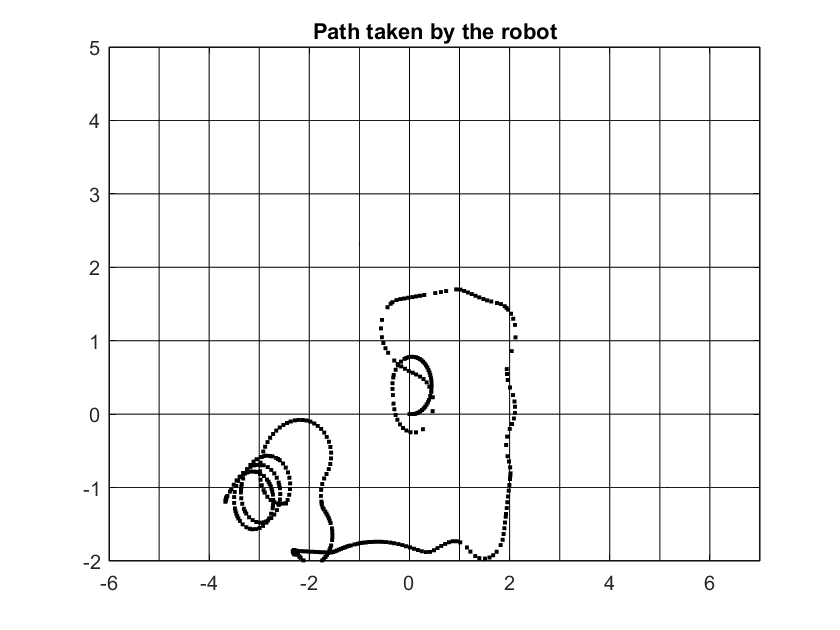
\includegraphics[width=0.5\textwidth]{../../images/squiggles2.png}}
    \caption{Plot from a spiral random walk algorithm implemented for floor cleaning robot}
    \label{fig10}
\end{figure}

The robot first starts spiral movements, and then when it hits an obstacle, it moves until it has enough space to start spiral movements again. 

\section{Ending Notes}
Overall the course Mobile Robotics was even more challenging than I estimated it to be. Especially coming from a computer science background and having so little knowledge about fundamental concepts such as feedback loop, it was a steep learning curve, but I loved every minute of this confusing journey because the peers in the course and the instructor have been extremely helpful and considerate throughout. The course was a proper learning journey from quizzes to the project, and I am grateful for sticking with the course to the end. 

\end{document}